\documentclass[11pt, a4paper]{article}
\usepackage[affil-it]{authblk} 
\usepackage{etoolbox}
\usepackage{lmodern}
\usepackage{titlesec}
\usepackage{float}

\makeatletter
\patchcmd{\@maketitle}{\LARGE \@title}{\fontsize{20}{19.2}\selectfont\@title}{}{}
\makeatother

\renewcommand\Authfont{\fontsize{16}{14.4}\selectfont}
\renewcommand\Affilfont{\fontsize{12}{10.8}\itshape}

\title{\textbf{Assignment 2}} 
\author{Pavan R Hebbar - 130010046}
\usepackage{graphicx}
\begin{document}
\maketitle
\newpage
\section{Question 1:}

The equation for normalised sheath potential is:

\begin{equation}
 \frac{d^2V}{d\eta^2} = \sqrt{\left(1+\frac{2V}{M_{se}^2}\right)} - e^{-V}
\end{equation}

The equation for the corresponding electric field is
\begin{equation}
 \frac{dV}{d\eta} = \sqrt{2M_{se}^2\left(\sqrt{\left(1+\frac{2V}{M_{se}^2}\right)}-1\right) + 2e^{-V} + \epsilon^2 - 2}
\end{equation}

For a neutral wall $M_{se}^2 = 1$

\section{Question 2:}
\subsection{Bohm's approximation}
For $V<<1$
\begin{equation}
 \frac{d^2V}{d\eta^2} = V\left(1-\frac{1}{M_{se}^2}\right)
\end{equation}
and
\begin{equation}
 \frac{dV}{d\eta} = \sqrt{\left(1 - \frac{1}{M_{se}^2}\right)V^2 + \epsilon^2}
\end{equation}
For a neutral wall $M_{se}^2 = 1$, implying $d^2V/d\eta = 0$ and $dV/d\eta = \epsilon$

\subsection{Child- Langmuir approximation:}
For $V>>1$
\begin{equation}
 \frac{d^2V}{d\eta^2} = \frac{M_{se}}{\sqrt{2}}\frac{1}{\sqrt{V}}
\end{equation}
and
\begin{equation}
 \frac{dV}{d\eta} = 2^{3/4}\sqrt{M_{se}}V^{1/4}
\end{equation}
For a neutral wall $M_{se}^2 = 1$.

\section{Question 3:}
The plots of normalised sheath potential are shown below for the 3 cases. $\epsilon = 0.01$ has been used.
\begin{figure}[H]
 \centering
 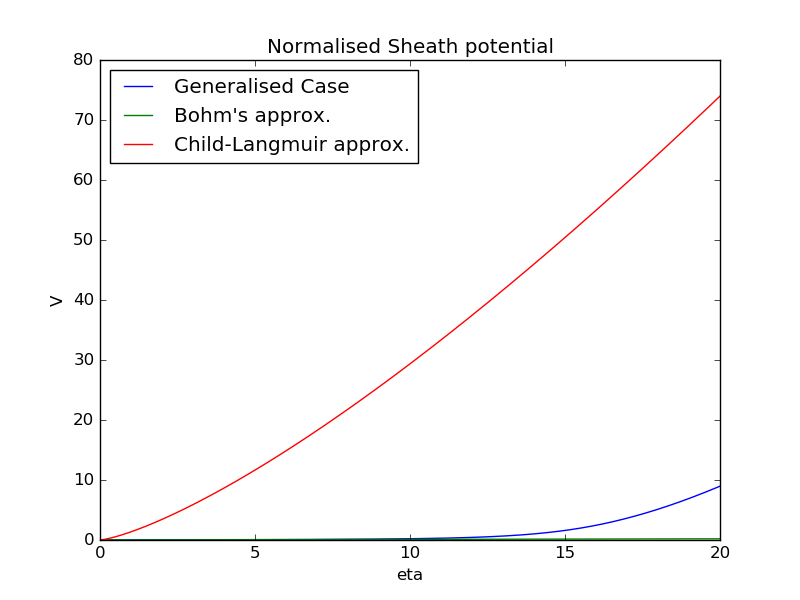
\includegraphics[scale = 0.5]{Gen_Vnorm.png}
\end{figure}

Plots of normalised electric field:
\begin{figure}[H]
 \centering
 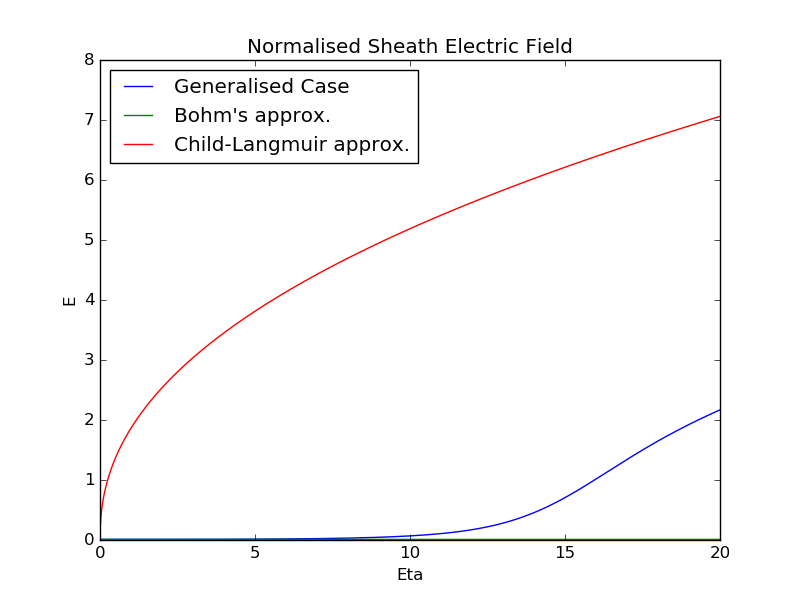
\includegraphics[scale = 0.5]{Gen_Enorm.png}
\end{figure}

\section{Question 4:}
We checked the normalised thickness of sheath for $dV/d\eta = 0.1, 0.01, 0.001$, we get a normalised sheath thickness($\eta$)
of $7.63, 16.32, 33.83$ respectively. Refer code ($\Delta eta = 0.01$)

\section{Question 5:}
We checked the values of $dV/d\eta$ at wall for $\epsilon$ values of $0.1, 0.01, 0.001$. The results are $1.1268, 1.1224, 1223$
respectively. Thus se can see the the values are very near to 1 and tend to 1 as we decrease the value of $\epsilon$

\section{Question 6:}
For electrode potential $= 1V$ sheath thickness(normalised) $= 14.29$\\
For electrode potential $= 10V$ sheath thickness(normalised) $= 21.14$\\
For electrode potential $= 100V$ sheath thickness(normalised) $= 47.04$\\
We see that for 1V and 10V, Bohm's approximation is always better than Child Langmuir approximation. For 100V, Child Langmuir
approximation is better for $\eta > 46.98$ ($\Delta eta = 0.01$)


\end{document}